\documentclass[11pt,a4paper]{article}

\usepackage[margin=1in, paperwidth=8.3in, paperheight=11.7in]{geometry}
\usepackage{amsmath,amsfonts,fancyhdr,bbm,tikz}
\usetikzlibrary{trees}
\usepackage[section,nohyphen]{DomH}
\headertitle{Financial Mathematics - Assessed Problem Sheet 3}

\begin{document}

\questionsfalse
% \answersfalse

\title{Financial Mathematics - Assessed Problem Sheet 3}
\author{Dom Hutchinson}
\date{\today}
\maketitle

\begin{question}{1. a)}
  A ``Down-and-Out Call'' with knockout price $b$ and rebate $R$ is an ordinary American call with strike price $K$ as long as the stock price does not fall below the knockout price. If the stock price falls below the knockout price at a random time point $t<T$, then the option expires and the owner of the option receives at time point $\tau$ the rebate $R$.
\end{question}

\begin{question}{1. a) i.}
  By defining an appropriate stopping time, give a mathematical description of the payoff of the down-and-out call. Find also a European claim that is equivalent to this claim.
\end{question}

\begin{answer}{1. a) i.}
  Define stopping time $\tau=\inf\{t:S_t\leq b\}$, this represents the first time the stock price falls below the knockout price $b$.
  \par The payoff process $\{Y_t\}$ for the Down-and-Out call can be expressed as
  \[ Y_t=\begin{cases}
  \{S_t-K\}_+&\text{if }t<\tau\\
  R&\text{if }t\geq\tau
  \end{cases} \]
  % TODO - Equivalent european claim
  Consider the European Claim $X=Y_\tau\frac{B_T}{B_\tau}$ which corresponds to exercising the Down-and-Out call at time $\tau$ and then accumulating interest from the bank account until the expiry date of the claim at time $T$.
\end{answer}

\begin{question}{1. a) ii.}
  Consider now a Cox-Ross-Rubinstein model with $T=3$ periods and stock price process $\{S_t\}$ where $S_0=80,u=3/2,d=1/2$ and interest rate $r=0.1$.
  \par Calculate the risk-neutral probability and the stock prices at each node in the tree.
\end{question}

\begin{answer}{1. a) ii.}
  Consider the tree below which shows the possible evolutions of the price process $S_t$ for each time-point and event.
  \begin{center}
    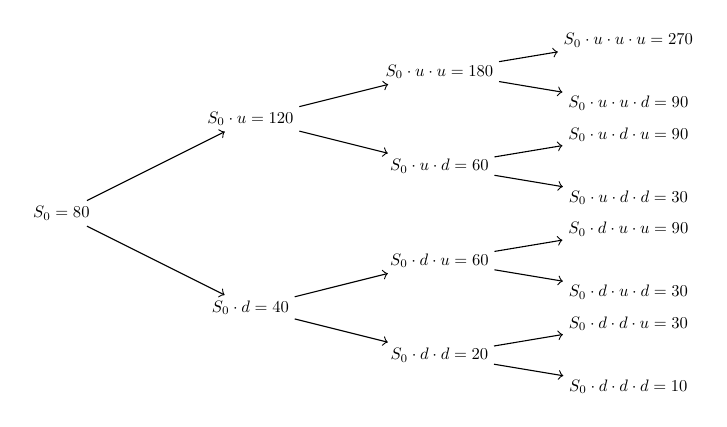
\begin{tikzpicture}[->, level/.style={sibling distance = 4cm/(#1), level distance = 4cm}, scale=0.6,transform shape,grow=right]
      \node {$S_0=80$}
        child {node {$S_0\cdot d=40$}
          child {
            node {$S_0\cdot d\cdot d=20$}
            child {node {$S_0\cdot d\cdot d\cdot d=10$}}
            child {node {$S_0\cdot d\cdot d\cdot u=30$}}
          }
          child {
            node {$S_0\cdot d\cdot u=60$}
            child {node {$S_0\cdot d\cdot u\cdot d=30$}}
            child {node {$S_0\cdot d\cdot u\cdot u=90$}}
          }
        }
        child {node {$S_0\cdot u=120$}
          child {
            node {$S_0\cdot u\cdot d=60$}
            child {node {$S_0\cdot u\cdot d\cdot d=30$}}
            child {node {$S_0\cdot u\cdot d\cdot u=90$}}
          }
          child {
            node {$S_0\cdot u\cdot u=180$}
            child {node {$S_0\cdot u\cdot u\cdot d=90$}}
            child {node {$S_0\cdot u\cdot u\cdot u=270$}}
          }
        };
    \end{tikzpicture}
  \end{center}
  The risk-neutral probability measure for a Cox-Ross-Rubinstein model satisfies
  \[ \Q(S_t=S_0u^nd^{t-n})={t\choose n}q^n(1-q)^{t-n}\text{ where }q=\frac{1+r-d}{u-d}\text{ for }n=0,\dots,t \]
  where $n$ is the number of up steps taken in the first $t$ time-periods.
  \par Under this specification of the Cox-Ross-Rubinstein model
  \[ q=\frac{1+0.1-0.5}{1.5-0.5}=\frac35 \]
  Thus
  \[ \Q(S_t=S_0u^nd^{t-n})={t\choose n}\frac{3^n2^{t-n}}{5^t}\text{ for }n=0,\dots,t \]
  By inspecting the tree of stock prices above we can determine the possible prices at each time-point, and thus the risk-neutral probability of each node.
  \par At time $t=0$
  \[\begin{array}{rcl}
    \Q(S_0=80)&=&\Q(S_0=S_0)=1
  \end{array}\]
  \par At time $t=1$
  \[\begin{array}{rcl}
    \Q(S_1=120)&=&\Q(S_1=S_0u)
    ={1\choose1}\cdot\frac35
    =\frac35\\
    \Q(S_1=40)&=&\Q(S_1=S_0d)
    ={1\choose0}\cdot\frac25
    =\frac25
  \end{array}\]
  At time $t=2$
  \[\begin{array}{rcl}
    \Q(S_2=180)&=&\Q(S_2=S_0u^2)
    ={2\choose2}\cdot\frac{3^2}{5^2}
    =\frac9{25}\\
    \Q(S_2=60)&=&\Q(S_2=S_0ud)
    ={2\choose1}\cdot\frac{3\cdot2}{5^2}
    =2\cdot\frac6{25}=\frac{12}{25}\\
    \Q(S_2=40)&=&\Q(S_2=S_0d^2)
    ={2\choose0}\cdot\frac{2^2}{5^2}
    =\frac4{25}
  \end{array}\]
  At time $t=3$
  \[\begin{array}{rclcl}
    \Q(S_3=270)&=&\Q(S_3=S_0u^3)
    &=&{3\choose3}\cdot\frac{3^3}{5^3}
    =\frac{27}{125}\\
    \Q(S_3=90)&=&\Q(S_3=S_0u^2d)
    &=&{3\choose2}\cdot\frac{3^2\cdot2}{5^3}
    =3\cdot\frac{18}{125}=\frac{54}{125}\\
    \Q(S_3=30)&=&\Q(S_3=S_0ud^2)
    &=&{3\choose1}\cdot\frac{3\cdot2^2}{5^3}
    =3\cdot\frac{12}{125}
    =\frac{36}{125}\\
    \Q(S_3=10)&=&\Q(S_3=S_03^3)
    &=&{3\choose0}\cdot\frac{2^3}{5^3}
    =\frac{8}{125}\\
  \end{array}\]
  I summarise these values in the tree below
  \begin{center}
    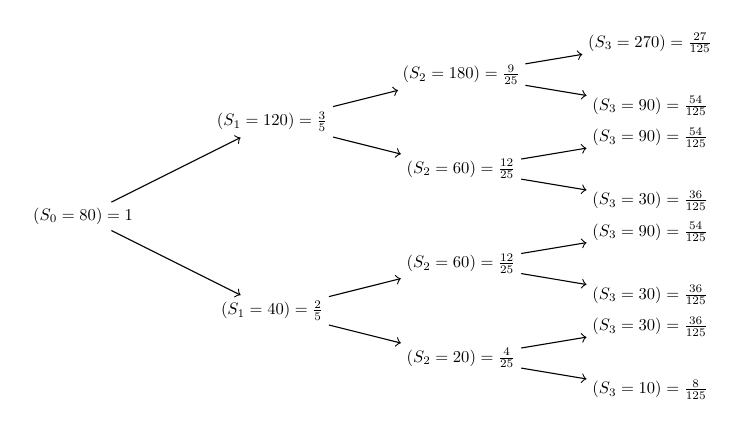
\begin{tikzpicture}[->, level/.style={sibling distance = 4cm/(#1), level distance = 4cm}, scale=0.6,transform shape,grow=right]
      \node {$\Q(S_0=80)=1$}
        child {node {$\Q(S_1=40)=\frac25$}
          child {
            node {$\Q(S_2=20)=\frac4{25}$}
            child {node {$\Q(S_3=10)=\frac8{125}$}}
            child {node {$\Q(S_3=30)=\frac{36}{125}$}}
          }
          child {
            node {$\Q(S_2=60)=\frac{12}{25}$}
            child {node {$\Q(S_3=30)=\frac{36}{125}$}}
            child {node {$\Q(S_3=90)=\frac{54}{125}$}}
          }
        }
        child {node {$\Q(S_1=120)=\frac35$}
          child {
            node {$\Q(S_2=60)=\frac{12}{25}$}
            child {node {$\Q(S_3=30)=\frac{36}{125}$}}
            child {node {$\Q(S_3=90)=\frac{54}{125}$}}
          }
          child {
            node {$\Q(S_2=180)=\frac9{25}$}
            child {node {$\Q(S_3=90)=\frac{54}{125}$}}
            child {node {$\Q(S_3=270)=\frac{27}{125}$}}
          }
        };
    \end{tikzpicture}
  \end{center}
\end{answer}

\begin{question}{1. a) iii.}
  Considering the same Cox-Ross-Rubinstein model, calculate the value of the down-and-out call with knockout price $b=70$, rebate $R=2$ and exercise price $K=120$ at every time point $t$ and for every state $\omega$.
  \par Then calculate a replicating strategy.
\end{question}

\begin{answer}{1. a) iii.}
  The tree below specifies the pay-out process $\{Y_t\}$ of the down-and-out call option is exercised at each possible time-point and sequence of events
  \begin{center}
    \begin{tikzpicture}[->, level/.style={sibling distance = 4cm/(#1), level distance = 4cm}, scale=0.6,transform shape,grow=right]
      \node {$\{80-120\}_+=0$}
        child {node {$R=2$}}
        child {node {$\{120-120\}_+=0$}
          child {node {$R=2$}}
          child {
            node {$\{180-120\}_+=60$}
            child {node {$\{90-120\}_+=0$}}
            child {node {$\{270-120\}_+=150$}}
          }
        };
    \end{tikzpicture}
  \end{center}
  I construct a Snell Envelope $\{Z_t\}$ to determine the the value of the down-and-out option at each time-point $t$ and state $\omega$.
  At time-point $t=3$
  \[ Z_3(\omega)=Y_3(\omega)\ \forall\ \omega \]
  At time-point $t=2$ and state $\omega_{uu}$ (ie Two up steps have occurred)
  \[ \expect[Z_3|\mathcal{F}_2]=\frac{1}{1.1}\left(150q+0\cdot(1-q)\right)=81.8182 \]
  At time-point $t=2$ and state $\omega_{ud}$ (ie One up step and one down step have occurred)
  \[ \expect[Z_3|\mathcal{F}_2]=\frac1{1.1}\left(2q+2\cdot(1-q)\right)=1.8182 \]
  At time-point $t=2$ and state $\omega_{dd}$ (ie Two down steps have occurred)
  \[ \expect[Z_3|\mathcal{F}_2]=\frac1{1.1}\left(2q+2\cdot(1-q)\right)=1.8182 \]
  Thus
  \[\begin{array}{rcl}
    Z_2(\omega)&=&\max(\expect[Z_3|\mathcal{F}_2],Y_2(\omega))\\
    &=&\begin{cases}
      \max(60,81.8182)&\text{if }\omega=\omega_{uu}\\
      \max(2,1.8182)&\text{otherwise}\\
    \end{cases}\\
    &=&\begin{cases}
      81.8182&\text{if }\omega=\omega_{uu}\\
      2&\text{otherwise}\\
    \end{cases}
  \end{array}\]
  At time-point $t=1$ and state $\omega_{u}$ (ie One up steps has occurred)
  \[ \expect[Z_2|\mathcal{F}_1]=\frac1{1.1}\left(81.8182\cdot q+2\cdot(1-q)\right=45.3554 \]
  At time-point $t=1$ and state $\omega_{d}$ (ie One down step has occurred)
  \[ \expect[Z_2|\mathcal{F}_1]=\frac1{1.1}\left(2q+2\cdot(1-q)\right)=1.8182 \]
  Thus
  \[\begin{array}{rcl}
    Z_1(\omega)&=&\max(\expect[Z_2|\mathcal{F}_1],Y_1(\omega))\\
    &=&\begin{cases}
      \max(45.3554,0)&\text{if }\omega=\omega_u\\
      \max(2,1.8182)&\text{if }\omega=\omega_d
    \end{cases}\\
    &=&\begin{cases}
      45.3554&\text{if }\omega=\omega_u\\
      2&\text{if }\omega=\omega_d
    \end{cases}
  \end{array}\]
  At time-point $t=0$
  \[\begin{array}{rcl}
    \expect[Z_1|\mathcal{F}_0]&=&\expect[Z_1]\\
    &=&\frac1{1.1}\left(45.3554\cdot q+2(1-q)\right)\\
    &=&25.4666
  \end{array}\]
  Thus
  \[ Z_0=\max(\expect[Z_1|\mathcal{F}_0],Y_0(\omega))=\max(25.4666,0)=25.4666 \]
  I summarise the value of this call option at each time-point and event in the tree below
  \begin{center}
    \begin{tikzpicture}[->, level/.style={sibling distance = 4cm/(#1), level distance = 4cm}, scale=0.6,transform shape,grow=right]
      \node {$Z_0=25.4665$}
        child {node {$Z_1(\omega_d)=2$}}
        child {node {$Z_1(\omega_u)=45.3554$}
          child {node {$Z_2(\omega_{ud})=2$}}
          child {
            node {$Z_2(\omega_{uu})=81.8182$}
            child {node {$Z_3(\omega_{uud})=0$}}
            child {node {$Z_3(\omega_{uuu})=150$}}
          }
        };
    \end{tikzpicture}
  \end{center}
  Using the optimal stopping theorem, the optimal stopping strategy $\{\tau(t)\}_t$ is
  \[\begin{array}{rcl}
    \tau(3)(\omega)&=&3\ \forall\ \omega\\
    \tau(2)(\omega)&=&\begin{cases}
      3&\text{if }\omega\in\{\omega_{uuu},\omega_{uud}\}\\
      2&\text{otherwise}
    \end{cases}\\
    \tau(1)(\omega)&=&\begin{cases}
      3&\text{if }\omega\in\{\omega_{uuu},\omega_{uud}\}\\
      2&\text{if }\omega\in\{\omega_{udu},\omega_{udd}\}\\
      1&\text{otherwise}
    \end{cases}\\
    \tau(0)(\omega)&=&\begin{cases}
      3&\text{if }\omega\in\{\omega_{uuu},\omega_{uud}\}\\
      2&\text{if }\omega\in\{\omega_{udu},\omega_{udd}\}\\
      1&\text{otherwise}
    \end{cases}\\
  \end{array}\]
  I now find a replicating strategy $\{H(t)\}$ for $\tau(0)$. In the third-time period the following equations must be satisfied
  \[\begin{array}{rrcl}
    &H_0(3)+270H_1(3)&=&Z_3(\omega_{uuu})=150\\
    &H_0(3)+90H_1(3)&=&Z_3(\omega_{uud})=0\\
    \implies&H_1(3)&=&\frac{150}{180}=\frac56\\
    \implies&H_0(3)&=&0-90\cdot\frac56=-75
  \end{array}\]
  Thus $H(3)(\omega)=(-75,5/6)$ if $\omega\in\{\omega_{uuu},\omega_uud\}$. We do not consider any other states as the option would have already been exercised by time-point $t=3$.
  \par In the second-time period the following equations must be satisfied
  \[\begin{array}{rrcl}
    &H_0(2)+180H_1(2)&=&Z_2(\omega_{uu})=81.8182\\
    &H_0(2)+60H_1(2)&=&Z_2(\omega_{ud})=2\\
    \implies&H_1(2)&=&\frac{79.8182}{120}=0.6652\\
    \implies&H_0(2)&=&2-60\cdot0.6651=-37.906
  \end{array}\]
  Thus $H(2)(\omega)=(-37.906,0.6652)$ if $\omega\in\{\omega_{uu},\omega_ud\}$. We do not consider any other states as the option would have already been exercised by time-point $t=2$.
  \par In the first-time period the following equations must be satisfied
  \[\begin{array}{rrcl}
    &H_0(1)+120H_1(1)&=&Z_1(\omega_{u})=45.3554\\
    &H_0(1)+40H_1(1)&=&Z_1(\omega_{d})=2\\
    \implies&H_1(1)&=&\frac{45.3554}{80}=0.5669\\
    \implies&H_0(1)&=&2-40\cdot0.5669=-20.676
  \end{array}\]
  Thus $H(1)(\omega)=(-20.676,0.5669)$ for all $\omega$.
\end{answer}

\begin{question}{1. a) iv.}
  Consider the same Cox-Ross-Rubinstein model and a usual European call option which matures at time $T=3$ with exercise price $K=120$. Calculate the time $t=0$ price and compare with the price of the down-and-out call.
\end{question}

\begin{answer}{1. a) iv.}
  The time $t=0$ of a European call option in a Cox-Ross-Rubinstein model is
  \[ \Pi(0)=\frac1{(1+r)^T}\sum_{n=0}^T{T\choose n}q^n(1-q)^{T-n}\{S_0u^nd^{T-n}-K\}_+ \]
  More specifically, for the model in this question, a European call option with exercise price $K=120$ and exercise date $T=3$
  \[\begin{array}{rcl}
    \Pi(0)&=&\frac1{1.1^3}\sum_{n=0}^3{3\choose n}\frac{3^n2^{3-n}}{5^3}\left\{80\cdot\frac{3^n\cdot1^{3-n}}{2^3}-120\right\}_+\\
    &=&\frac1{1.1^3}\bigg\{{3\choose 0}\cdot\frac{2^3}{5^3}\{10-120\}_++{3\choose 1}\cdot\frac{3\cdot2^2}{5^3}\{30-120\}_+\\
    &&+{3\choose 2}\cdot\frac{3^2\cdot2}{5^3}\{90-120\}_++{3\choose 3}\cdot\frac{3^3}{5^3}\{270-120\}_+\bigg\}\\
    &=&\frac1{1.1^3}\cdot\frac{3^3}{5^3}\cdot150\\
    &=&24.34259\dots
  \end{array}\]
  This is less valuable than the down-and-out call.
\end{answer}

\begin{question}{1. b) i.}
  Find the probability that standard Brownian Motion lies between some values $a,b$, with $a\leq b$, at time $T$, in terms of the normal distribution function $\Phi$.
  \par Find the expected value of $\exp\{cW_T\}\ \forall\ c\in\reals$.
\end{question}

\begin{answer}{1. b) i.}
  Let $a\leq b$ and $\{W_t\}_t$ be standard Brownian motion.
  \par Note that $W_T\sim\text{Normal}(0,T)$, thus $\frac1{\sqrt{T}}W_T\sim\Phi$.
  Thus
  \[\begin{array}{rcl}
    \prob(W_T\in[a,b])&=&\prob(W_T\leq b)-\prob(W_T\leq a)\\
    &=&\prob\left(\frac1{\sqrt{T}}W_T\leq\frac{b}{\sqrt{T}}\right)-\prob\left(\frac1{\sqrt{T}}W_T\leq\frac{a}{\sqrt{T}}\right)\\
    &=&\Phi(b/\sqrt{T})-\Phi(a/\sqrt{T})
  \end{array}\]
  Consider the expected value of $e^{cW_T}$ for $c\in\reals$
  \[\begin{array}{rcl}
    \expect\left[e^{cW_T}\right]&=&\int e^{cx}f_{W_T}(x)dx\\
    &=&\int e^{cx}\cdot\frac1{\sqrt{2\pi T}}e^{-\frac12\cdot\frac{x^2}T}dx\\
    &=&\int\frac1{\sqrt{2\pi T}}\exp\left\{-\frac12\cdot\frac{(x-c)^2+c^2}T\right\}dx\\
    &=&e^{c^2/T}\int\frac1{\sqrt{2\pi T}}\exp\left\{-\frac12\cdot\frac{(x-c)^2}T\right\}dx\\
    &=&e^{c^2/T}\cdot\expect\left[\text{Normal}(c,T)\right]\\
    &=&ce^{c^2/T}
  \end{array}\]
\end{answer}

\begin{question}{1. b) ii.}
  Consider two independent standard Brownian motions $W_t^{(1)}$ and $W_t^{(2)}$ and write the linear combination
  \[ X_t=\gamma W_t^{(1)}+\sqrt{1-\gamma^2}W_t^{(2)} \]
   where $\gamma\in[-1,1]$ is a constant. Show that $X_t$ is a standard Brownian Motion.
\end{question}

\begin{answer}{1. b) ii.}
  Let $\{W_t^{(1)}\}_t\{W_t^{(2)}\}$ be independent standard Brownian motions and define stochastic process $\{X_t\}_t$ as
  \[ X_t=\gamma W_t^{(1)}+W_t^{(2)}\sqrt{1-\gamma^2}\text{ with }\gamma\in[-1,1] \]
  There are four properties I need to show for $X_t$ to be a standard Brownian motion
  \begin{enumerate}
    \item \textit{That $X_0=0$.}
    \[\begin{array}{rcl}
      X_0&=&\gamma W_0^{(1)}+W_t^{(2)}\sqrt{1-\gamma^2}\\
      &=&\gamma\cdot0+0\cdot\sqrt{1-\gamma^2}\\
      &=&0
    \end{array}\]
    $X_t$ has this property.

    \item \textit{Increments of $X_t$ are independent.}
    \par Consider the increment $(X_{t+u}-X_t)$ for $t,u\geq0$
    \[\begin{array}{rcl}
      (X_{t+u}-X_t)&=&\left(\gamma W_{t+u}^{(1)}+W_{t+u}^{(2)}\sqrt{1-\gamma^2}\right)-\left(\gamma W_{t}^{(1)}+W_{t}^{(2)}\sqrt{1-\gamma^2}\right)\\
      &=&\gamma(W_{t+u}^{(1)}-W_t^{(1)})+\sqrt{1-\gamma^2}(W_{t+u}^{(1)}-W_t^{(1)})
    \end{array}\]
    Since $W_t^{(1)},W_t^{(2)}$ are standard Brownian motions then their increments $(W_{t+u}^{(1)}-W_t^{(1)}),(W_{t+u}^{(2)}-W_t^{(2)})$ are both independent of $\mathcal{F}_t$. Thus, by linearity the increment of $X_t$ is independent of $\mathcal{F}_t$.

    \item \textit{$X_t$ has stationary Gaussian increments.}
    \par Consider the increment $(X_{t+u}-X_t)$ for $t,u\geq0$
    \[ (X_{t+u}-X_t)=\gamma(W_{t+u}^{(1)}-W_t^{(1)})+\sqrt{1-\gamma^2}(W_{t+u}^{(1)}-W_t^{(1)}) \]
    As the increments of $W_t^{(1)},W_t^{(2)}$ have gaussian distributions, the increments of $X_t$ have gaussian distributions to. Now consider the mean and variance of these increments
    \[\begin{array}{rcl}
      \expect[X_{t+u}-X_t]&=&\gamma\expect[W_{t+u}^{(1)}-W_t^{(1)}]+\sqrt{1-\gamma^2}\expect[W_{t+u}^{(2)}-W_t^{(2)}]\\
      &=&\gamma\cdot0+\sqrt{1-\gamma^2}\cdot0\\
      &=&0\\\\
      \var[X_{t+u}-X_t]&=&\gamma^2\var[W_{t+u}^{(1)}-W_t^{(1)}]+(\sqrt{1-\gamma^2})^2\var[W_{t+u}^{(2)}-W_t^{(2)}]\\
      &=&\gamma^2\cdot u+(1-\gamma^2)u\\
      &=&u
    \end{array}\]
    Thus
    \[ (X_{t+u}-X_t)\sim\text{Normal}(0,u)\text{ for all }t,u\geq0 \]

    \item \textit{$X_t$ has continuous paths.}
    \par We know that $W_t^{(1)}(\omega),W_t^{(2)}(\omega)$ are continuous functions of $t$ for all $\omega$.
    \par Thus, by linearity, $X_t(\omega)$ is a continuous function of $t$ for all $\omega$.
  \end{enumerate}
  Since $X_t$ has all four properties, it is a standard Brownian motion.
\end{answer}

\end{document}
